\subsection{Документ <<Выработка гофроагрегата>>}
\label{doc:corrugatorproduction}



\subsubsection{Описание предметной области}

Документ существует в СИСТЕМЕ.
Документ предназначен для регистрации выработки заготовок и готовой продукции на гофроагрегате. Является рабочим местом оператора гофроагрегата.
Документ участвует в процессе "Выпуск готовой продукции и полуфабрикатов".



 \subsubsection{Функциональные требования}


\point{Исправить проверку выполнения задания}

При проверке выполнения данного задания, должна проверять  выполнение задания из значения ''Процент выпуска'' технологической карты заказа , а в случае если полученное значение равно «0» брать значение по умолчанию из настроек Системы.


\point{Печатать внутренней бирки}

Внутренняя бирка на заготовки должна печататься из СИСТЕМЫ.
За основу необходимо взять печатную форму СИСТЕМЫ и внести правки.
%привести к тому виду, который сейчас используется на ПРЕДПРИЯТИИ. 
Внешний вид внутренней бирки для заготовок представлен на рис. \ref{pic:InnerLabel}.

Бирки необходимо распечатать как для всех позиций выработки, так и для выделенных строк.

Бирка должна содержать следующие поля:
\begin{itemize}
    \item Номер заказа в СИСТЕМЕ;
    \item Наименование заготовки;
    % \item Размеры заготовки;
    \item Наименование номенклатуры готовой продукции;
    \item Контрагент;
    \item Дата производства, время начала выполнения заказа;
    % \item Оборудование;
    \item Номер смены.
    % \item Количество на паллете;
    % \item Марка + Профиль + Цвет.
\end{itemize}

%Реквизиты организации должны выводиться исходя из организации, указанной для заказа.

%На бирку (внутрицеховая) добавить время выпуска, номер (идентификатор) и № ярлыка по порядку с общим количеством ярлыков на этот заказ (например, 3 / 25). 
% На бирке выводить время печати (оно заменяет время выпуска, которое может быть еще неизвестно к моменту печати), идентификатор задания (из НП) и  № ярлыка с общим количеством ярлыков по данному раскрою (например, 3 из 25). Нумерация ярлыков должна идти с единицы для каждого раскроя с этим заказом (т.е., если будет два задания, то номера в бирках будут с единицы в обоих случаях).

\begin{figure*}[!htb]
\centering
  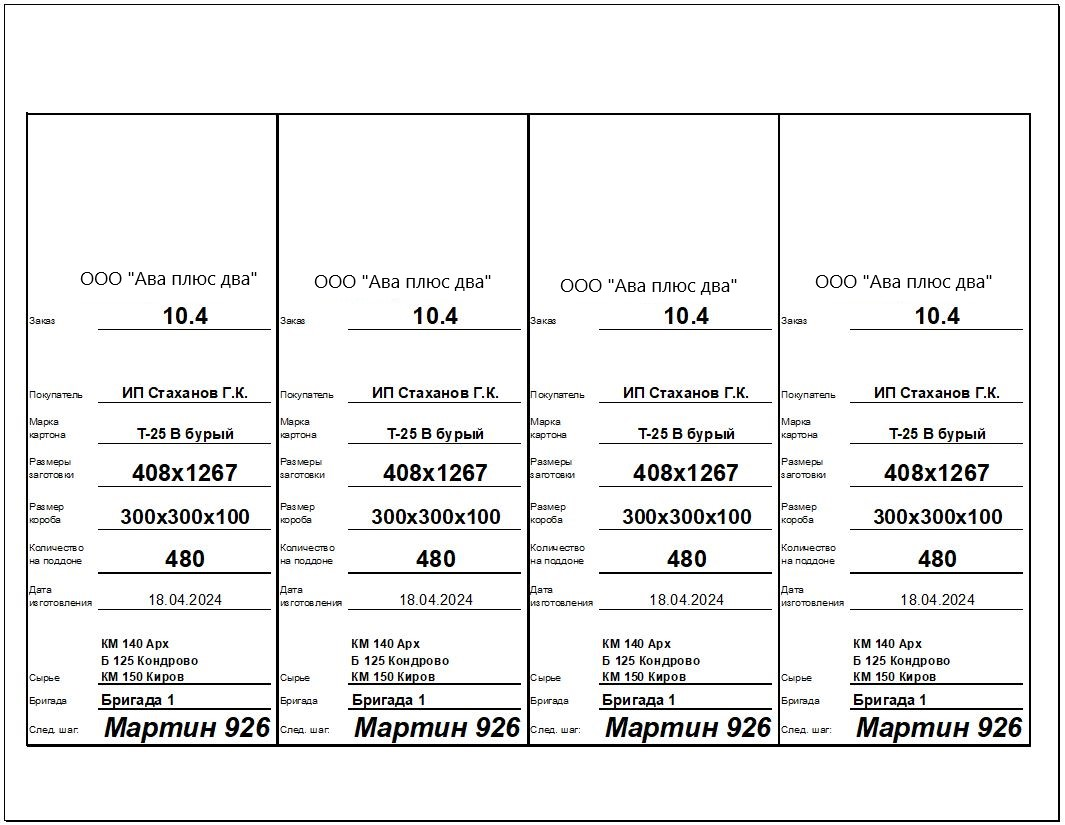
\includegraphics[width=140mm, height=220mm, keepaspectratio]{50_Pics/InnerLabel.JPG}
\caption{Пример внутренней бирки с гофроагрегата}
\label{pic:InnerLabel}
\end{figure*} 
\FloatBarrier







\point{Печать бирки на готовую продукцию}
\label{print:label}


Бирка на готовую продукцию (товарный гофрокартон) должна печататься из СИСТЕМЫ.
% %Добавить возможность печати бирок из СИСТЕМЫ.
% При печати бирок на готовую продукцию необходимо печатную форму привести к тому виду, который сейчас используется на ПРЕДПРИЯТИИ.

Пример бирки на товарный гофрокартон представлен на рис. \ref{pic:Label}.
% Графа с номером паллеты остается пустой и должна заполняться в распечатанном бланке упаковщиком.

% Реквизиты организации должны выводиться исходя из организации, указанной для заказа.
Бирка должна содержать следующие поля:
\begin{itemize}
    \item Наименование и адрес организации;
    % \item Логотип организации;
    \item Тип изделия. Значение определяется во типу продукции свойства ''Тип продукции'' в типе изделия технологической карты;
    \item Наименование номенклатуры;
    % \item Оборудование - оборудование последнего передела;
    \item Размер изделия;
    \item ГОСТ;
    \item Номер партии (??? не вывести);
    
    \item Бригада;
    % \item Цвет картона;
    % \item Марка картона;
    \item Количество на поддоне;
    \item Количество в кипе;
    \item Количество в партии;
    
    \item Штрих-код;
    % \item Манипуляционные знаки;
    % \item Количество на поддоне;
    % \item Количество подонов в заказе;
    % \item Марка картона;
    % \item Цвет картона;
    % \item Наименование линии;
    % \item Номер смены;
    \item Дата текущей выработки;
    % \item Дата первой выработки по заказу;
    % \item Номер заказа: Номер заказа в СИСТЕМЕ + Дата заказа + Номер заказа SAP + номер строки в SAP;
    % \item Номер паллеты в заказе;
    % \item Уникальный номер паллеты.
    % \item Тех.карта;
  %  \item Покупатель;
  %  \item Количество на поддоне;
  %  \item Бригада;
  %  \item Краткое наименование варианта упаковки, указанного в технологической карте.
\end{itemize}

Штрих-код на паллете должен определяться как номер заказа и количество продукции в паллете.


\begin{figure*}[!htb]
\centering
  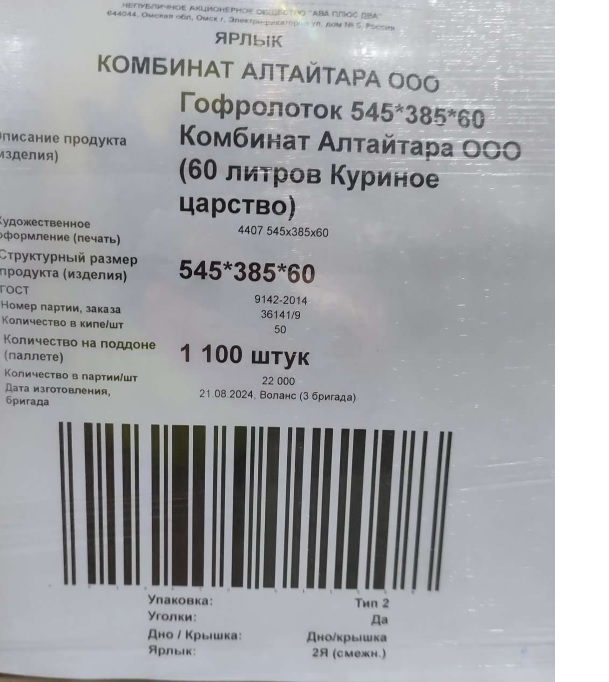
\includegraphics[width=140mm, height=220mm, keepaspectratio]{50_Pics/Label.jpg}
\caption{Пример бирки готовую продукцию}
\label{pic:Label}
\end{figure*} 
\FloatBarrier

% Поле <<Номер заказа в СИСТЕМЕ>> обозначено на примере цифрами 6693, поле <<Тех.карта>> обозначено на примере цифрами 1608.


ШК-код содержит строку формата: 
\begin{itemize}
    \item Код заказа 6 символов; % 4146500;
    % \item Символ ";"
    % \item "0000";
    % \item Первая часть номера заказа 6 знаков (номер заказа SAP);
    % \item Вторая часть заказа произвосдтва (номер строки в заказе SAP) 6 знаков с ведущими нулями;
    \item Количество на паллете 6 знаков с ведущими нулями;
    % \item Дата производства в формате ГГГГММДД.
\end{itemize}

Пример строки: 401465001100.